The warm interface electronics %must 
provide an interface between the \dword{ce}, \dword{daq}, timing, and slow control systems, including local power control at the flange and a real-time diagnostic readout. They are housed in the \dwords{wiec} attached directly to the \dword{ce} flange.  The \dword{wiec} shown in Figure~\ref{fig:tpcelec-flange} 
contains one power and timing card (\dword{ptc}), five warm interface boards (\dwords{wib}) and a passive
power and timing backplane (PTB), which fans out signals and \dword{lv} power from the \dword{ptc} to the \dwords{wib}. The \dword{wiec} must provide a Faraday-shielded housing, robust ground connections from the \dwords{wib} to the detector ground described in Section~\ref{sec:fdsp-tpc-elec-design-ground}, and only optical fiber links to the \dword{daq} and slow control in order to mitigate noise introduced at the \dword{ce} \fdth.


\begin{dunefigure}
[Exploded view of the \dword{ce} signal flange for \dword{pdsp}.]
{fig:tpcelec-flange}
{Exploded view of the \dword{ce} signal flange for \dword{pdsp}.  The design will be very similar for the \dword{spmod} \dword{ce} signal flange (with two \dword{ce} signal flanges per \fdth).}
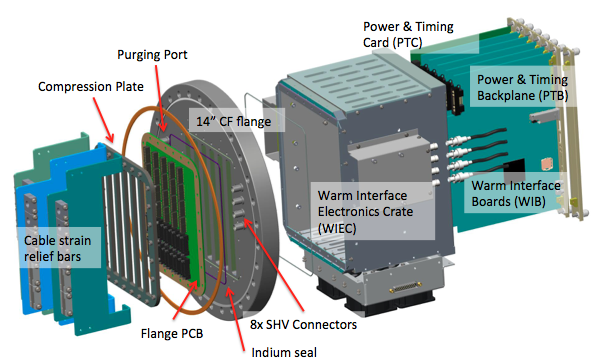
\includegraphics[width=0.9\linewidth]{tpcelec-flange.png}
\end{dunefigure}

The \dword{wib} is the interface between the \dword{daq} system and four
\dwords{femb}. It receives the system clock and control signals from the
timing system and provides for processing and fan-out of those signals to the four
\dwords{femb}. The \dword{wib} also receives the high-speed data signals from the four 
\dwords{femb} and transmits them to the \dword{daq} system over optical
fibers. The data signals are recovered onboard the \dword{wib} with commercial equalizers.
The \dwords{wib} are attached directly to the TPC
\dword{ce} \fdth on the signal flange. The \fdth
board is a PCB with connectors to the cold signal and \dword{lv} power cables fitted
between the compression plate on the cold side, and sockets for
the \dword{wib} on the warm side. Cable strain relief for the cold cables is 
supported from the back end of the \fdth.

\begin{dunefigure}
[\dword{pdsp} PTC and timing distribution to the WIB and FEMBs]
{fig:tpcelec-wib_timing}
{Power and timing card (\dword{ptc}) and timing distribution to the \dword{wib} and \dwords{femb} used in \dword{pdsp}.}
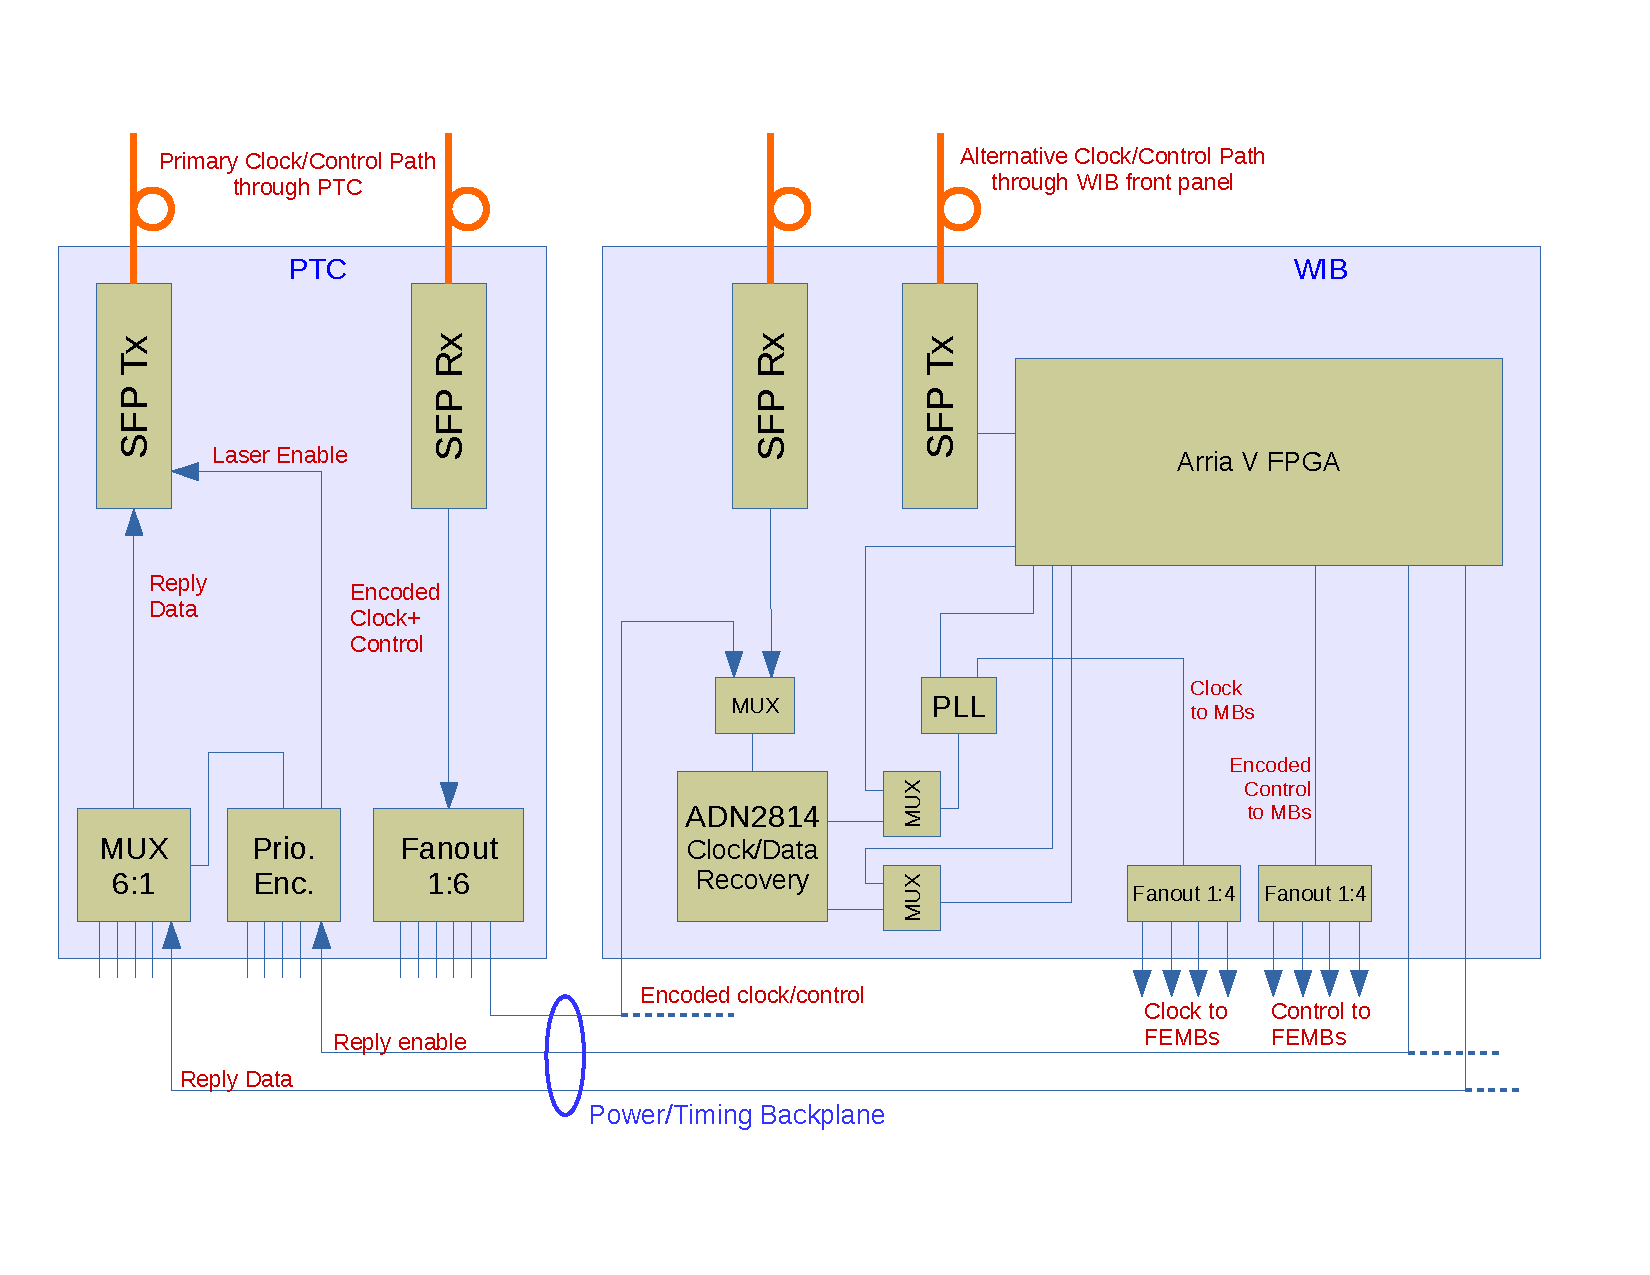
\includegraphics[width=0.75\linewidth]{tpcelec-wib_timing.pdf}
\end{dunefigure}

The \dword{pdsp} \dword{ptc} provides a bidirectional fiber interface to the
timing system. The clock and data
streams are separately fanned out to the five \dwords{wib} as shown in
Figure~\ref{fig:tpcelec-wib_timing}. The \dword{ptc} fans the clocks out to the \dword{wib} over the
PTB, which is a passive backplane attached directly to the \dword{ptc} and
\dwords{wib}.  The received clock on the \dword{wib} is separated into clock and
data using a clock-data separator. Timing endpoint firmware to receive and transmit
the clock is integrated in the \dword{wib} \dword{fpga} (the Altera Arria V\footnote{Altera Arria\texttrademark{}, V FPGA family, \url{https://www.altera.com/products/fpga/arria-series/arria-v/overview.html}.} was used for \dword{pdsp}).
The \dword{spmod} timing system, described in Section~\ref{sec:fdsp-daq-timing}, is a development of the \dword{pdsp} system, and expected to require the nearly identical functionality at the \dword{wib} endpoint.

\begin{dunefigure}
[\dword{pdsp} \dword{lv} power distribution to the \dword{wib} and \dwords{femb}]
{fig:tpcelec-wib_power}
{\dword{lv} power distribution to the \dword{wib} and \dwords{femb} implemented for \dword{pdsp}. This will be modified for the \dword{spmod} to provide the required voltage or voltages depending on which \dwords{asic} are used on the \dwords{femb}. In particular the voltages to the \dword{femb} \numrange{0}{3} will change as the \dword{pdsp} \dword{fpga} is replaced by \dword{coldata}. }
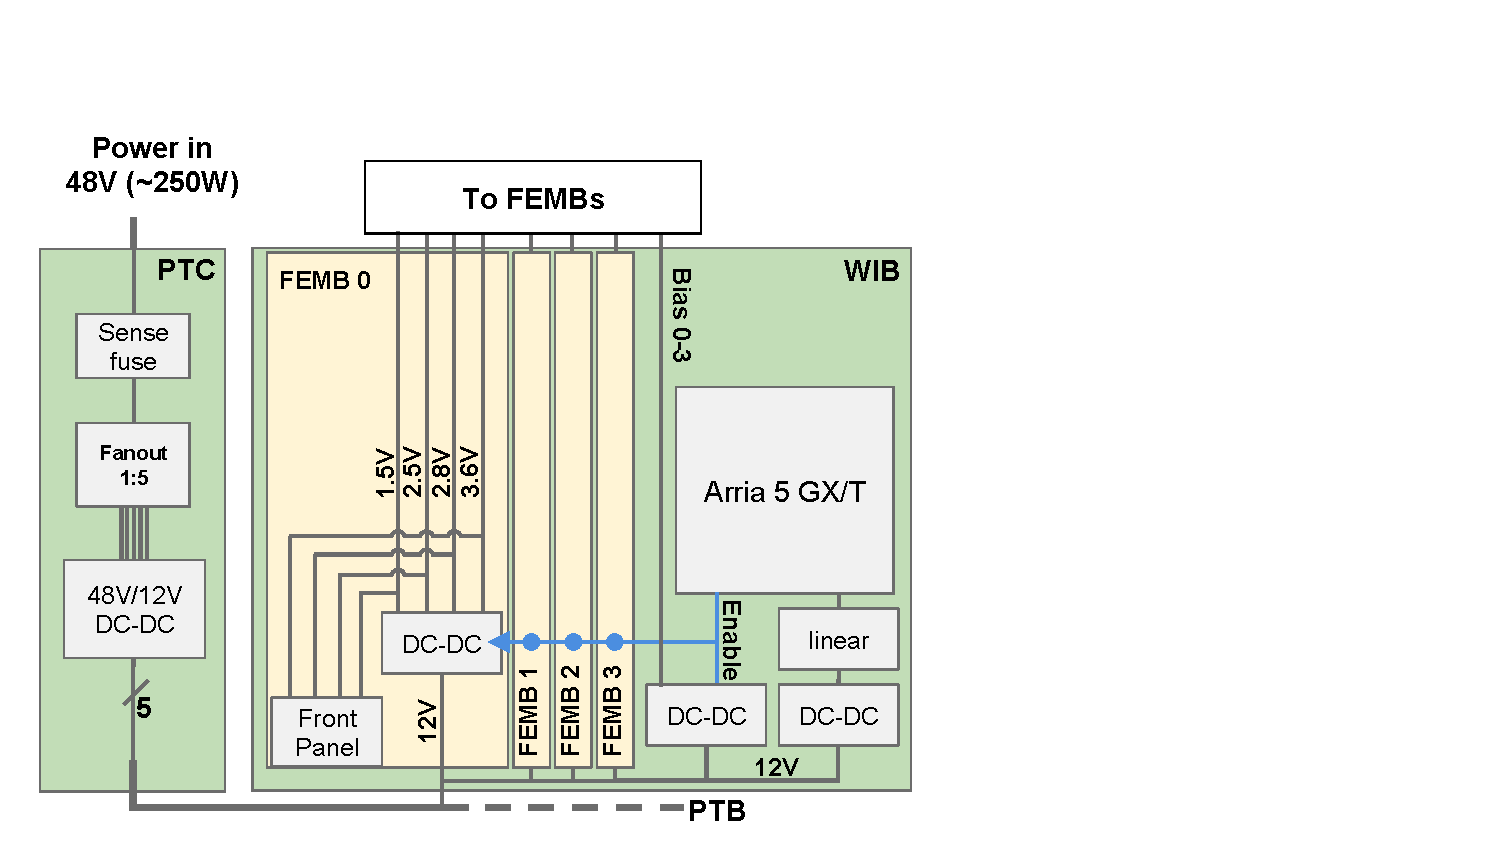
\includegraphics[width=0.65\linewidth]{tpcelec-wib_power.pdf}
\end{dunefigure}


The \dword{ptc} also receives \SI{48}{V} \dword{lv} power for all cold
electronics connected through the TPC signal flange: one \dword{ptc}, five \dword{wib}, and \num{20}~\dword{femb}. The \dword{lv} power is then stepped down
to \SI{12}{V} via a DC-DC converter onboard the \dword{ptc}. The output of the \dword{ptc} converters is filtered with a common-mode choke and fanned out
on the PTB to each \dword{wib}, which provides the necessary \SI{12}{V} DC-DC conversions and fans
the \dword{lv} power out to each of the cold \dwords{femb} supplied by that \dword{wib}, 
as shown in Figure~\ref{fig:tpcelec-wib_power}. The output of the \dword{wib} converters are further filtered by a common-mode choke. The 
majority of the power drawn by a full flange is dissipated in the \lar by the cold \dword{femb}.

%Each \dword{wib} contains a 
%unique IP address for its UDP slow control interface. The IP address for the \dword{wib} is 
%derived from a crate and slot address: the crate address is generated on the \dword{ptc} 
%board via dipswitches and the slot address is generated by the PTB slot, numbered 
%from one to five. Note that the \dwords{wib} also have front-panel
%connectors for receiving \dword{lv} power; these can be used in place of 
%the \dword{lv} power inputs on the PTB generated by the \dword{ptc}.

As shown in Figure~\ref{fig:tpcelec-dune_wib}, the \dword{wib} is capable of receiving \dword{lv} power in the front panel and distributing it directly to the \dword{femb}, bypassing all DC/DC converters.
It can also receive the encoded system timing signals over bi-directional optical
fibers on the front panel, and process these using either
the on-board \dword{fpga} or clock synthesizer chip to provide the clock required by the \dword{ce}.
The baseline \dword{asic} design currently uses 8b/10b encoding; if the SLAC CRYO \dword{asic} is selected for
the DUNE \dword{spmod}, 12b/14b encoding will be used instead of 8b/10b.

%\begin{dunefigure}


The \dword{fpga} on the \dword{pdsp} \dword{wib} is an Altera Arria V GT variant, which has
transceivers that can drive the high-speed data to the \dword{daq} system up to
10.3125~Gbps per link, implying that all data from
two \dword{femb} (2$\times$5~Gbps) could be transmitted on a single link.
The \dword{fpga} has an additional Gbps Ethernet transceiver I/O based on the \SI{125}{MHz} clock, which 
provides real-time digital data readout to the slow control system.
